\section{Gradient Descent and the Ghost of Soviet Planning (The Present)}

\subsection{From Learning to Control: The LeCunian Synthesis}

As deep learning matured, a curious convergence began to take shape—one that returned to the roots of physical reasoning and optimization. Among its most vocal advocates was Yann LeCun, who argued that the future of artificial intelligence lay not just in larger models, but in reframing them through the lens of \textbf{control theory}.

Neural networks, LeCun observed, could be interpreted not merely as function approximators, but as \textit{dynamical systems} evolving toward optimal behavior. Training, in this view, becomes a feedback loop. Each weight update is a control action; each activation, a transient state; each gradient, a signal of how far the system has deviated from its objective.

This reinterpretation is not just mathematically elegant—it’s philosophically profound. Control theory offers a unifying framework that links the behavior of intelligent machines with the natural evolution of systems under constraints. It provides not only a formalism for optimization, but a language for agency, intention, and adaptation.

Let us now explore this convergence. From Kepler’s ellipses to Pontryagin’s Hamiltonians, from gradient descent to backpropagation, we arrive at a view of machine learning as \textbf{optimal control over information landscapes}.

\subsection{From Celestial Mechanics to Machine Learning: Control as a Unifying Lens}

Just as Kepler’s Second Law revealed structure in planetary motion, the training dynamics of a neural network reveal structure in the flow of representations. Both describe systems evolving under constraint—guided not by chance, but by optimization. Where classical mechanics traced orbits through force and momentum, machine learning traces abstractions through weights and gradients. In both cases, there is a path, and that path is not arbitrary.

Control theory provides a framework for understanding this evolution—whether in physical systems or artificial ones. Where Kepler’s ellipse emerged from a variational principle in mechanics, a neural network’s trajectory through weight space arises from an optimization over function space. The mathematics is different in symbol, but not in essence.

At the heart of both domains lie the same structures: the \textbf{Lagrangian}, describing the tradeoff between potential and kinetic energy; and the \textbf{Hamiltonian}, encoding the total structure of the system’s evolution. In a neural network, there is no literal mass or motion, but there is an analogous form of energy—expressed in the loss function. The loss captures the system’s tension between representation and error, and its gradients act like generalized forces, guiding the network’s evolution toward a more efficient internal state.

From this perspective, training a neural network becomes a modern instance of \textbf{optimal control theory}. The forward pass is a state trajectory \( x(t) \), the weights \( u(t) \) are control inputs, and the backpropagated gradients \( p(t) \) serve as costates. The learning objective—the loss—is the integral to be minimized, and the \textbf{Pontryagin Hamiltonian} forms the core structure guiding this evolution.

Just as we reinterpreted Kepler’s laws through control theory, we can now reinterpret neural learning through the same lens. Optimization, dynamics, and intention are not exclusive to physics. They are alive in machine intelligence. Let us now see how.

\subsection{Neural Networks as Discretized Control Systems: Learning in the Language of Action}

In deep learning, the architecture of a neural network can be viewed as a discretized control system:

\begin{itemize}
  \item \( x(t) \): the activation (state) at layer or time \( t \)
  \item \( u(t) \): the weights (control input) we adjust
  \item \( f(x, u) \): the forward pass dynamics
  \item \( p(t) \): the backpropagated gradient (costate)
  \item \( J \): the loss we minimize
\end{itemize}


\begin{figure}[H]
\centering
\begin{tikzpicture}[node distance=2cm and 2.8cm, on grid, auto, >=stealth', thick]

  % Forward states x(t)
  \foreach \i in {0,...,3} {
    \node[draw, circle, minimum size=1.4cm] (x\i) at (3*\i, 0) {\(x_{\i}\)};
  }

  % Controls u(t)
  \foreach \i in {0,...,2} {
    \node[draw, rectangle, minimum width=1.6cm, minimum height=1cm, fill=blue!10] (u\i) at (3*\i+1.5, 2.8) {\(u_{\i}\)};
  }

  % Backpropagation nodes p(t)
  \foreach \i in {1,...,3} {
    \node[draw, circle, minimum size=1.4cm, fill=red!10] (p\i) at (3*\i, 5.8) {\(p_{\i}\)};
  }

  % Forward arrows (x(t+1) = f(x,u))
  \foreach \i in {0,...,2} {
    \draw[->] (x\i) -- node[midway, below] {\(f(x_{\i}, u_{\i})\)} (x\the\numexpr\i+1);
    \draw[->] (u\i) -- (x\the\numexpr\i+1);
  }

% Backward arrows (costate evolution)
\foreach \i in {1,...,2} {
  \draw[->, dashed, red!60!black] 
    (p\the\numexpr\i+1) -- 
    node[pos=0.5, sloped, above] {\(\nabla_x \mathcal{H}\)} 
    (p\i);
}


  % Feedback to controls
  \foreach \i in {0,...,2} {
    \draw[->, dashed, blue!60!black] (p\the\numexpr\i+1) to[bend right=30] node[midway, left] {\(\nabla_u \mathcal{H}\)} (u\i);
  }

  % Loss node
  \node[above=1.8cm of p3] (loss) {\(J = \text{Loss}(x_3)\)};
  \draw[->, dashed] (loss) -- (p3);

  % Labels aligned vertically on the left
  \node at (-2.5, 5.8) {\textbf{Backpropagation}};
  \node at (-2.5, 2.8) {\textbf{Control Inputs}};
  \node at (-2.5, 0) {\textbf{Forward Pass}};

\end{tikzpicture}
\caption{Training as Optimal Control: States \(x(t)\), controls \(u(t)\), gradients \(p(t)\), and the Hamiltonian loop under Pontryagin’s principle. The learning process forms a cycle of forward dynamics, backward feedback, and optimal control.}
\end{figure}

Here too, we can define a Hamiltonian, derive adjoint equations, and optimize weights via local maximization. The entire learning process becomes a Pontryagin-like loop: forward dynamics, backward gradients, and a maximization step.


In this view, \textbf{training a deep neural network is optimal control over function space}. Just as entropy measures what we do not know, and mutual information measures what we learn, Pontryagin’s framework measures how we act under those constraints to achieve a goal.

\begin{quote}
\emph{If entropy is the geometry of uncertainty, then Pontryagin’s Maximum Principle is its compass.}
\end{quote}

In a world governed by constraints, noise, and feedback, optimal control becomes the engine that transforms information into action. And at the heart of it all lies the same ancient tool: integration—not of rectangles, but of meaning across time.



In the optimal control view of deep learning, the components of a neural network training loop map directly onto elements of a dynamical control system. Each has a role in guiding the system from initial conditions to an optimal state that minimizes a given objective. Below, we unpack the interpretation of each variable.

\subsection{\(\mathbf{x}(t)\): The Activation (State)}

The variable \(\mathbf{x}(t)\) represents the full state of the system at discrete time step or layer \(t\). In a neural network, this corresponds not to a single neuron, but to the **entire vector of activations** across all neurons in that layer. These activations encode the transformed representations of the input data as they propagate forward through the network.

From the control systems perspective, \(\mathbf{x}(t)\) is analogous to a **state vector** that might include quantities like position and velocity in a physical system. Just as the state of a mechanical system evolves over time due to applied forces (control inputs), the hidden representations in a neural network evolve due to the transformations applied by the weights and nonlinearities. Each \(\mathbf{x}(t)\) is the result of applying the forward dynamics \(f(\mathbf{x}(t{-}1), \mathbf{u}(t{-}1))\), where \(\mathbf{u}(t{-}1)\) denotes the weights at the previous layer.

This control-theoretic view allows us to treat the neural network as a dynamical system where information flows forward layer by layer, and the evolving hidden states represent increasingly abstract features. Training then becomes the process of adjusting the controls \(\mathbf{u}(t)\) to steer the system through useful representations toward an optimal output.

\begin{figure}[H]
\centering
\begin{tikzpicture}[scale=1, every node/.style={transform shape}, node distance=1.6cm and 0.6cm]

  % Layers: input, hidden1, hidden2, output
  \foreach \i in {1,2,3} {
    \node[circle, draw, minimum size=1cm] (input\i) at (0, -\i*1.6) {};
    \node[circle, draw, minimum size=1cm, fill=blue!10] (h1\i) at (2.5, -\i*1.6) {};
    \node[circle, draw, minimum size=1cm] (h2\i) at (5, -\i*1.6) {};
    \node[circle, draw, minimum size=1cm] (output\i) at (7.5, -\i*1.6) {};
  }

  % Input -> Hidden1
  \foreach \i in {1,2,3} {
    \foreach \j in {1,2,3} {
      \draw[->, thick] (input\i) -- (h1\j);
    }
  }

  % Hidden1 -> Hidden2
  \foreach \i in {1,2,3} {
    \foreach \j in {1,2,3} {
      \draw[->, thick] (h1\i) -- (h2\j);
    }
  }

  % Hidden2 -> Output
  \foreach \i in {1,2,3} {
    \foreach \j in {1,2,3} {
      \draw[->, thick] (h2\i) -- (output\j);
    }
  }

  % State labels x(t) above everything
  \node[above=1.2cm of input1] {\(\mathbf{x}(0)\)};
  \node[above=1.2cm of h11] {\(\mathbf{x}(1)\)};
  \node[above=1.2cm of h21] {\(\mathbf{x}(2)\)};
  \node[above=1.2cm of output1] {\(\mathbf{x}(3)\)};

  % Layer labels below x(t)
  \node[above=0.4cm of input1] {Input Layer};
  \node[above=0.4cm of h11] {Hidden Layer 1};
  \node[above=0.4cm of h21] {Hidden Layer 2};
  \node[above=0.4cm of output1] {Output Layer};

  % Caption under figure
  \node at (3.75, -6.2) {\small \textit{Each \(\mathbf{x}(t)\) represents the full activation state across all neurons at layer \(t\).}};

\end{tikzpicture}
\caption{A neural network as a layered dynamical system. At each layer \(t\), the state \(\mathbf{x}(t)\) is a vector of neuron activations, evolving through the network via learned dynamics.}
\end{figure}


\paragraph{Example.} Suppose layer \( t = 1 \) has three neurons, and the corresponding activation vector is:
\[
\mathbf{x}(1) = 
\begin{bmatrix}
0.2 \\
0.8 \\
0.1
\end{bmatrix}
\]
This vector represents the internal state of the network at layer 1. Each element in \( \mathbf{x}(1) \) corresponds to the activation of a neuron at that layer. These values are the result of applying the transformation \( f(\mathbf{x}(0), \mathbf{u}(0)) \), and they serve as input to the next transformation \( f(\mathbf{x}(1), \mathbf{u}(1)) \) to produce \( \mathbf{x}(2) \).

In this interpretation, the neural network evolves its internal representation — the state vector — step-by-step through each layer, just like a physical system evolves over time in response to control inputs.


\begin{figure}[H]
\centering
\begin{tikzpicture}[scale=1, every node/.style={transform shape}, node distance=1.6cm and 0.6cm]

  % Coordinates for x positions
  \def\xInput{0}
  \def\xHidOne{2.5}
  \def\xHidTwo{5}
  \def\xOut{7.5}

  % Coordinates for y positions
  \def\yOne{-1.6}
  \def\yTwo{-3.2}
  \def\yThree{-4.8}

  % Input layer nodes
  \node[circle, draw, minimum size=1cm] (input1) at (\xInput, \yOne) {};
  \node[circle, draw, minimum size=1cm] (input2) at (\xInput, \yTwo) {};
  \node[circle, draw, minimum size=1cm] (input3) at (\xInput, \yThree) {};

  % Hidden layer 1 nodes with example values
  \node[circle, draw, fill=blue!20, minimum size=1cm] (h1) at (\xHidOne, \yOne) {\textcolor{red}{0.2}};
  \node[circle, draw, fill=blue!20, minimum size=1cm] (h2) at (\xHidOne, \yTwo) {\textcolor{red}{0.8}};
  \node[circle, draw, fill=blue!20, minimum size=1cm] (h3) at (\xHidOne, \yThree) {\textcolor{red}{0.1}};

  % Hidden layer 2
  \node[circle, draw, minimum size=1cm] (h21) at (\xHidTwo, \yOne) {};
  \node[circle, draw, minimum size=1cm] (h22) at (\xHidTwo, \yTwo) {};
  \node[circle, draw, minimum size=1cm] (h23) at (\xHidTwo, \yThree) {};

  % Output layer
  \node[circle, draw, minimum size=1cm] (out1) at (\xOut, \yOne) {};
  \node[circle, draw, minimum size=1cm] (out2) at (\xOut, \yTwo) {};
  \node[circle, draw, minimum size=1cm] (out3) at (\xOut, \yThree) {};

  % Connections (simplified for clarity)
  \foreach \i in {1,2,3} {
    \foreach \j in {1,2,3} {
      \draw[->, thick] (input\i) -- (h\j);
      \draw[->, thick] (h\j) -- (h2\j);
      \draw[->, thick] (h2\j) -- (out\j);
    }
  }

  % Layer boxes (state space boundaries) - manually sized
  \draw[dashed, thick, gray!50] ($(input3)+(-0.7,-0.7)$) rectangle ($(input1)+(0.7,0.7)$);
  \draw[dashed, thick, gray!50] ($(h3)+(-0.7,-0.7)$) rectangle ($(h1)+(0.7,0.7)$);
  \draw[dashed, thick, gray!50] ($(h23)+(-0.7,-0.7)$) rectangle ($(h21)+(0.7,0.7)$);
  \draw[dashed, thick, gray!50] ($(out3)+(-0.7,-0.7)$) rectangle ($(out1)+(0.7,0.7)$);


  % Labels for state spaces
  \node[above=1.2cm of input1] {\(\mathbf{x}(0)\)};
  \node[above=1.2cm of h1] {\(\mathbf{x}(1)\)};
  \node[above=1.2cm of h21] {\(\mathbf{x}(2)\)};
  \node[above=1.2cm of out1] {\(\mathbf{x}(3)\)};

  \node[below=0.7cm of input3, align=center] {\footnotesize\shortstack{State\\Space}};
  \node[below=0.7cm of h3, align=center] {\footnotesize\shortstack{Hidden\\Representation}};
  \node[below=0.7cm of h23, align=center] {\footnotesize\shortstack{Hidden\\Representation}};
  \node[below=0.7cm of out3, align=center] {\footnotesize\shortstack{Output\\Representation}};

  % Caption
  \node at (3.75, 1.5) {\small \textit{Example activation vector \(\mathbf{x}(1) = [0.2,\, 0.8,\, 0.1]^T\) shown in red, across the neurons in Hidden Layer 1.}};

\end{tikzpicture}
\caption{Layer-wise state evolution. Each dashed box represents a state space, with activations \(\mathbf{x}(t)\) evolving through learned dynamics.}
\end{figure}



\subsection{\(\mathbf{u}(t)\): The Weights (Control Input)}

The function \(\mathbf{u}(t)\) denotes the **control input** at discrete time or layer \(t\)—specifically, the collection of **weights and biases** that govern how the neural network transforms activations from one layer to the next. These are the trainable parameters that the learning algorithm seeks to optimize.

In the language of control theory, \(\mathbf{u}(t)\) is the actuator: the mechanism by which we steer the system from its current state \(\mathbf{x}(t)\) toward a desired future state \(\mathbf{x}(t+1)\). Through the function \(f(\mathbf{x}(t), \mathbf{u}(t))\), the network applies its current set of weights to process the activations and produce the next state. 

Just as a spacecraft adjusts its thrusters to follow a trajectory, a neural network adjusts its weights to follow an optimal transformation pathway—refining internal representations toward a lower loss. These weights are not fixed; they are updated iteratively using gradients propagated backward from the final loss \(J\), making the learning process a **feedback-driven control loop**.

\begin{figure}[H]
\centering
\begin{tikzpicture}[scale=1, every node/.style={transform shape}, node distance=1.6cm and 0.6cm]

  % Coordinates for x positions
  \def\xHidOne{0}
  \def\xHidTwo{2.5}

  % Y positions for neurons
  \def\yOne{-1.6}
  \def\yTwo{-3.2}
  \def\yThree{-4.8}

  % Hidden layer 1 nodes
  \node[circle, draw, fill=blue!10, minimum size=1cm] (h1) at (\xHidOne, \yOne) {};
  \node[circle, draw, fill=blue!10, minimum size=1cm] (h2) at (\xHidOne, \yTwo) {};
  \node[circle, draw, fill=blue!10, minimum size=1cm] (h3) at (\xHidOne, \yThree) {};

  % Hidden layer 2 nodes
  \node[circle, draw, fill=blue!5, minimum size=1cm] (h21) at (\xHidTwo, \yOne) {};
  \node[circle, draw, fill=blue!5, minimum size=1cm] (h22) at (\xHidTwo, \yTwo) {};
  \node[circle, draw, fill=blue!5, minimum size=1cm] (h23) at (\xHidTwo, \yThree) {};

  % Connections representing u(t)
  \foreach \i in {1,2,3} {
    \foreach \j in {1,2,3} {
      \draw[->, thick, blue!80] (h\i) -- (h2\j);
    }
  }

  % Bounding boxes for layers
  \draw[dashed, thick, gray!50] ($(h3)+(-0.7,-0.7)$) rectangle ($(h1)+(0.7,0.7)$);
  \draw[dashed, thick, gray!50] ($(h23)+(-0.7,-0.7)$) rectangle ($(h21)+(0.7,0.7)$);

  % Labels for x(t) and x(t+1)
  \node[above=1.2cm of h1] {\(\mathbf{x}(t)\)};
  \node[above=1.2cm of h21] {\(\mathbf{x}(t+1)\)};

  % Label for control input
  \node at (1.25, -0.3) {\textbf{\(\mathbf{u}(t)\): weights}};
  \draw[->, thick, blue!80] (1.25, -0.6) -- (1.25, -1.3);

  % Caption
  \node at (1.25, -6.2) {\small \textit{The control input \(\mathbf{u}(t)\) determines how \(\mathbf{x}(t)\) evolves into \(\mathbf{x}(t+1)\) via learned weights.}};

\end{tikzpicture}
\caption{Weights as control inputs. Each \(\mathbf{u}(t)\) contains the parameters that determine the transformation from \(\mathbf{x}(t)\) to \(\mathbf{x}(t+1)\). These connections form the mechanism by which the system acts.}
\end{figure}


\paragraph{Example.} Suppose the weights \(\mathbf{u}(1)\) from layer 1 to layer 2 are given by the following \(3 \times 3\) matrix:
\[
\mathbf{u}(1) =
\begin{bmatrix}
0.1 & 0.4 & 0.3 \\
0.7 & 0.2 & 0.6 \\
0.3 & 0.5 & 0.9
\end{bmatrix}
\]
and the activation vector from the previous layer is
\[
\mathbf{x}(1) = 
\begin{bmatrix}
0.2 \\
0.8 \\
0.1
\end{bmatrix}.
\]
The forward pass from layer 1 to layer 2 is a linear transformation followed by a nonlinearity:
\[
\mathbf{x}(2) = \sigma\left(\mathbf{u}(1) \cdot \mathbf{x}(1)\right),
\]
where \(\sigma(\cdot)\) is an elementwise activation function such as ReLU.

Computing the pre-activation:
\[
\mathbf{z}(2) = \mathbf{u}(1) \cdot \mathbf{x}(1) =
\begin{bmatrix}
0.1 & 0.4 & 0.3 \\
0.7 & 0.2 & 0.6 \\
0.3 & 0.5 & 0.9
\end{bmatrix}
\begin{bmatrix}
0.2 \\
0.8 \\
0.1
\end{bmatrix}
=
\begin{bmatrix}
0.1(0.2) + 0.4(0.8) + 0.3(0.1) \\
0.7(0.2) + 0.2(0.8) + 0.6(0.1) \\
0.3(0.2) + 0.5(0.8) + 0.9(0.1)
\end{bmatrix}
=
\begin{bmatrix}
0.41 \\
0.38 \\
0.64
\end{bmatrix}
\]
Applying \(\sigma\) (e.g., ReLU), we get:
\[
\mathbf{x}(2) = 
\begin{bmatrix}
0.41 \\
0.38 \\
0.64
\end{bmatrix}.
\]

In this way, the weights \(\mathbf{u}(1)\) act as the control input that determines how the system’s state evolves from \(\mathbf{x}(1)\) to \(\mathbf{x}(2)\).



\begin{figure}[H]
\centering
\begin{tikzpicture}[scale=1.1, every node/.style={transform shape}, node distance=1.6cm and 0.6cm]

  % Layer positions (increased horizontal distance)
  \def\xLeft{0}
  \def\xRight{7.0}

  % Y positions for neurons (doubled vertical spacing)
  \def\yOne{-2.0}
  \def\yTwo{-6.0}
  \def\yThree{-10.0}

  % x(1) nodes
  \node[circle, draw, fill=blue!15, minimum size=1cm] (a1) at (\xLeft, \yOne) {};
  \node[circle, draw, fill=blue!15, minimum size=1cm] (a2) at (\xLeft, \yTwo) {};
  \node[circle, draw, fill=blue!15, minimum size=1cm] (a3) at (\xLeft, \yThree) {};

  % x(2) nodes
  \node[circle, draw, fill=blue!5, minimum size=1cm] (b1) at (\xRight, \yOne) {\scriptsize 0.41};
  \node[circle, draw, fill=blue!5, minimum size=1cm] (b2) at (\xRight, \yTwo) {\scriptsize 0.38};
  \node[circle, draw, fill=blue!5, minimum size=1cm] (b3) at (\xRight, \yThree) {\scriptsize 0.64};

  % Connections with weights as labels
  \draw[->, thick, blue!80] (a1) -- node[midway, above, sloped, font=\scriptsize, blue] {0.1} (b1);
  \draw[->, thick, blue!80] (a2) -- node[near end, above, sloped, font=\scriptsize, blue] {0.4} (b1);
  \draw[->, thick, blue!80] (a3) -- node[near end, above, sloped, font=\scriptsize, blue] {0.3} (b1);

  \draw[->, thick, blue!80] (a1) -- node[near start, above, sloped, font=\scriptsize, blue] {0.7} (b2);
  \draw[->, thick, blue!80] (a2) -- node[near start, above, sloped, font=\scriptsize, blue] {0.2} (b2);
  \draw[->, thick, blue!80] (a3) -- node[near start, above, sloped, font=\scriptsize, blue] {0.6} (b2);

  \draw[->, thick, blue!80] (a1) -- node[near end, above, sloped, font=\scriptsize, blue] {0.3} (b3);
  \draw[->, thick, blue!80] (a2) -- node[near start, above, sloped, font=\scriptsize, blue] {0.5} (b3);
  \draw[->, thick, blue!80] (a3) -- node[midway, above, sloped, font=\scriptsize, blue] {0.9} (b3);

  % Labels
  \node[above=1.2cm of a1] {\(\mathbf{x}(1)\)};
  \node[above=1.2cm of b1] {\(\mathbf{x}(2)\)};
  \node at (3.5, -1.0) {\(\mathbf{u}(1)\) (weights)};
  \node at (3.5, -11.4) {\small \textit{Weight-labeled connections compute \(\mathbf{x}(2) = \sigma(\mathbf{u}(1) \cdot \mathbf{x}(1))\)}};

\end{tikzpicture}
\caption{Example of control input \(\mathbf{u}(1)\) acting on \(\mathbf{x}(1)\) to produce \(\mathbf{x}(2)\). Weights appear as labeled edges; resulting activations are shown inside right-side neurons.}
\end{figure}






\subsection{\(f(x, u)\): The Forward Dynamics}

The function \(f(x, u)\) governs the **forward dynamics** of the system: it describes how the state \(\mathbf{x}(t)\) evolves into the next state \(\mathbf{x}(t+1)\), given the current control input \(\mathbf{u}(t)\). In neural networks, this corresponds to a layer’s transformation: typically a **linear mapping** (weights and biases) followed by a **nonlinear activation function** such as ReLU, tanh, or softmax.

From a control-theoretic standpoint, \(f(x, u)\) plays the role of the system’s **update rule**—the equivalent of the laws of motion in a dynamical system. It defines how current information is processed to produce the next state. From an information-processing view, it is the internal mechanism that encodes, compresses, filters, or amplifies features as they propagate forward.

In deep learning, this function is not fixed; it is shaped during training by adjusting the parameters \(u(t)\). Yet, at each moment of evaluation, \(f(x, u)\) represents a **fixed and deterministic flow**: given \(x(t)\) and \(u(t)\), the output is fully determined. This deterministic processing across layers defines the **architecture's semantics**—the rules by which abstract representations are learned.

Just as in physics, where the trajectory of a body depends on both its current state and applied forces, in neural networks, the evolution of internal representations depends jointly on current activations and the applied weights.

\begin{figure}[H]
\centering
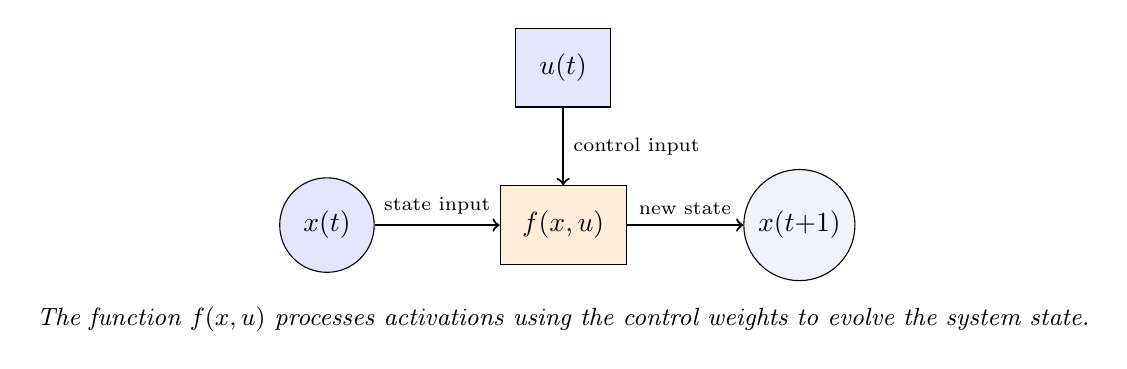
\begin{tikzpicture}[scale=1, every node/.style={transform shape}, node distance=2cm and 2cm]

  % Node positions
  \node[circle, draw, fill=blue!10, minimum size=1.2cm] (x) at (0,0) {\(x(t)\)};
  \node[rectangle, draw, fill=orange!15, minimum width=1.6cm, minimum height=1cm] (f) at (3,0) {\(f(x, u)\)};
  \node[circle, draw, fill=blue!5, minimum size=1.2cm] (xnext) at (6,0) {\(x(t{+}1)\)};
  \node[rectangle, draw, fill=blue!10, minimum width=1.2cm, minimum height=1cm] (u) at (3,2) {\(u(t)\)};

  % Arrows
  \draw[->, thick] (x) -- node[above, font=\scriptsize] {state input} (f);
  \draw[->, thick] (u) -- node[right, font=\scriptsize] {control input} (f);
  \draw[->, thick] (f) -- node[above, font=\scriptsize] {new state} (xnext);

  % Labels
  \node at (3, -1.2) {\small \textit{The function \(f(x, u)\) processes activations using the control weights to evolve the system state.}};

\end{tikzpicture}
\caption{Forward dynamics \(f(x, u)\) as the processing engine of the network. It combines the current state and control to generate the next activation state.}
\end{figure}


\paragraph{Example.} The forward dynamics function \(f(x, u)\) encapsulates both the linear transformation and the nonlinearity that define how information flows through the network.

Suppose the activation vector and weight matrix are given as:
\[
\mathbf{x}(1) = 
\begin{bmatrix}
0.2 \\
0.8 \\
0.1
\end{bmatrix}, \quad
\mathbf{u}(1) =
\begin{bmatrix}
0.1 & 0.4 & 0.3 \\
0.7 & 0.2 & 0.6 \\
0.3 & 0.5 & 0.9
\end{bmatrix}.
\]

Then the forward dynamics at time \( t = 1 \) are computed via:
\[
\mathbf{x}(2) = f(\mathbf{x}(1), \mathbf{u}(1)) = \sigma(\mathbf{u}(1) \cdot \mathbf{x}(1)).
\]

First, compute the linear transformation:
\[
\mathbf{z}(2) = \mathbf{u}(1) \cdot \mathbf{x}(1) =
\begin{bmatrix}
0.1(0.2) + 0.4(0.8) + 0.3(0.1) \\
0.7(0.2) + 0.2(0.8) + 0.6(0.1) \\
0.3(0.2) + 0.5(0.8) + 0.9(0.1)
\end{bmatrix}
=
\begin{bmatrix}
0.41 \\
0.38 \\
0.64
\end{bmatrix}.
\]

Next, apply a nonlinearity such as ReLU:
\[
\mathbf{x}(2) = \sigma(\mathbf{z}(2)) = 
\begin{bmatrix}
\text{ReLU}(0.41) \\
\text{ReLU}(0.38) \\
\text{ReLU}(0.64)
\end{bmatrix}
=
\begin{bmatrix}
0.41 \\
0.38 \\
0.64
\end{bmatrix}.
\]

Thus, the function \(f(\mathbf{x}(1), \mathbf{u}(1))\) transforms the current state into the next, encoding both the weights and the activation function as part of the system's evolution rule.






\begin{figure}[H]
\centering
\begin{tikzpicture}[every node/.style={transform shape}, node distance=2cm and 1cm, font=\small]

  % Input vector x(1)
  \node[circle, draw, fill=blue!15, minimum size=1cm] (x1) at (0, 2) {\(0.2\)};
  \node[circle, draw, fill=blue!15, minimum size=1cm] (x2) at (0, 0) {\(0.8\)};
  \node[circle, draw, fill=blue!15, minimum size=1cm] (x3) at (0, -2) {\(0.1\)};
  \node[above=0.5cm of x1] {\(\mathbf{x}(1)\)};

  % Weight matrix U(1)
  \node[rectangle, draw, fill=blue!5, minimum width=1.4cm, minimum height=3.8cm] (U) at (2.5, 0) {\(\mathbf{u}(1)\)};
  \node[below=0.3cm of U] {Linear};

  % Output of matrix mult
  \node[circle, draw, fill=orange!10, minimum size=1cm] (z1) at (5, 2) {\(0.41\)};
  \node[circle, draw, fill=orange!10, minimum size=1cm] (z2) at (5, 0) {\(0.38\)};
  \node[circle, draw, fill=orange!10, minimum size=1cm] (z3) at (5, -2) {\(0.64\)};
  \node[above=0.5cm of z1] {\(\mathbf{z}(2)\)};

  % Activation function
  \node[rectangle, draw, fill=gray!10, minimum width=1.4cm, minimum height=3.8cm] (sigma) at (7.5, 0) {\(\sigma\)};
  \node[below=0.3cm of sigma] {ReLU};

  % Output x(2)
  \node[circle, draw, fill=blue!10, minimum size=1cm] (y1) at (10, 2) {\(0.41\)};
  \node[circle, draw, fill=blue!10, minimum size=1cm] (y2) at (10, 0) {\(0.38\)};
  \node[circle, draw, fill=blue!10, minimum size=1cm] (y3) at (10, -2) {\(0.64\)};
  \node[above=0.5cm of y1] {\(\mathbf{x}(2)\)};

  % Arrows
  \foreach \i in {1,2,3} {
    \draw[->, thick] (x\i) -- (U);
    \draw[->, thick] (U) -- (z\i);
    \draw[->, thick] (z\i) -- (sigma);
    \draw[->, thick] (sigma) -- (y\i);
  }

  % Caption
  \node at (5, -3.5) {\footnotesize \textit{Forward dynamics: \(\mathbf{x}(2) = \sigma(\mathbf{u}(1) \cdot \mathbf{x}(1))\)}};

\end{tikzpicture}
\caption{The function \(f(\mathbf{x}(1), \mathbf{u}(1))\) as a composition of linear transformation and nonlinearity. The activation vector is transformed by weights and passed through ReLU to produce the next state.}
\end{figure}






\subsection{\(\mathbf{p}(t)\): The Backpropagated Gradient (Costate)}

The variable \(\mathbf{p}(t)\) represents the \textbf{costate} in the language of optimal control—an invisible but powerful force that flows \textbf{backward through time}, guiding how the system should have behaved to achieve its objective.

In the context of deep learning, this corresponds to the \textbf{backpropagated error signal} at layer \(t\). It tells each layer how much its current state \(\mathbf{x}(t)\) contributed to the final loss \(J\), and therefore how that state should change to improve future outcomes. In essence, \(\mathbf{p}(t)\) is the \textbf{value of information} at time \(t\), quantified in terms of how sensitive the loss is to changes in the activation.

From a geometric perspective, \(\mathbf{p}(t)\) can be seen as a \textbf{gradient vector field} over the state space, pointing in the direction that most effectively improves the loss if we could nudge the current state. In control theory, the costate is derived from the Hamiltonian and obeys its own differential (or difference) equation—just like momentum in physics or shadow prices in economics.

Unlike the forward dynamics \(f(\mathbf{x}, \mathbf{u})\), which evolve deterministically given weights and activations, the costate evolution is \textbf{feedback-driven}: it originates at the final loss and ripples backward, layer by layer, encoding how each state contributes to that final outcome.

\medskip
\noindent
Put simply:
\begin{itemize}
  \item \(\mathbf{x}(t)\) tells us where the system is,
  \item \(\mathbf{u}(t)\) decides how we move forward,
  \item \(\mathbf{p}(t)\) tells us how much being at \(\mathbf{x}(t)\) “matters” for reaching our goal.
\end{itemize}

This backward feedback is what enables \textbf{learning}. It is the mechanism by which the network corrects itself—learning what to emphasize, what to suppress, and what pathways in the representation space are worth investing in.



\begin{figure}[H]
\centering
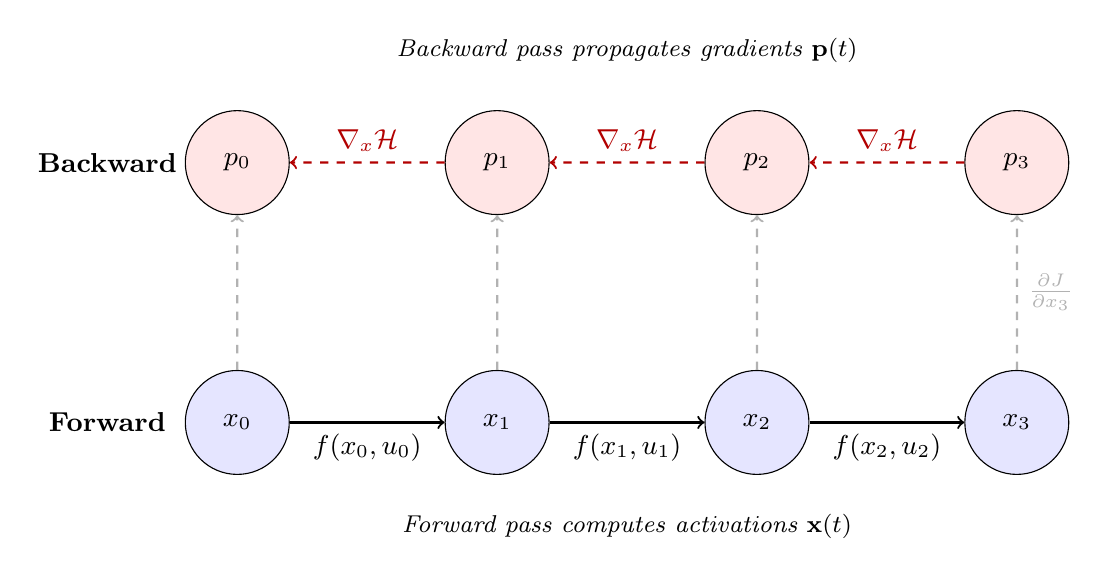
\begin{tikzpicture}[scale=1.1, every node/.style={transform shape}, node distance=1.6cm and 0.6cm, font=\small]

  % Node positions (forward path)
  \node[circle, draw, fill=blue!10, minimum size=1.2cm] (x0) at (0,0) {\(x_0\)};
  \node[circle, draw, fill=blue!10, minimum size=1.2cm] (x1) at (3,0) {\(x_1\)};
  \node[circle, draw, fill=blue!10, minimum size=1.2cm] (x2) at (6,0) {\(x_2\)};
  \node[circle, draw, fill=blue!10, minimum size=1.2cm] (x3) at (9,0) {\(x_3\)};

  % Costates (backward path)
  \node[circle, draw, fill=red!10, minimum size=1.2cm] (p3) at (9,3) {\(p_3\)};
  \node[circle, draw, fill=red!10, minimum size=1.2cm] (p2) at (6,3) {\(p_2\)};
  \node[circle, draw, fill=red!10, minimum size=1.2cm] (p1) at (3,3) {\(p_1\)};
  \node[circle, draw, fill=red!10, minimum size=1.2cm] (p0) at (0,3) {\(p_0\)};

  % Forward arrows
  \draw[->, thick] (x0) -- node[below] {\(f(x_0, u_0)\)} (x1);
  \draw[->, thick] (x1) -- node[below] {\(f(x_1, u_1)\)} (x2);
  \draw[->, thick] (x2) -- node[below] {\(f(x_2, u_2)\)} (x3);

  % Backward arrows (costate evolution)
  \draw[->, thick, dashed, red!70!black] (p3) -- node[above] {\(\nabla_x \mathcal{H}\)} (p2);
  \draw[->, thick, dashed, red!70!black] (p2) -- node[above] {\(\nabla_x \mathcal{H}\)} (p1);
  \draw[->, thick, dashed, red!70!black] (p1) -- node[above] {\(\nabla_x \mathcal{H}\)} (p0);

  % Vertical connections (loss-based feedback)
  \draw[->, thick, dashed, gray!60] (x3) -- node[right] {\(\frac{\partial J}{\partial x_3}\)} (p3);
  \draw[->, thick, dashed, gray!60] (x2) -- (p2);
  \draw[->, thick, dashed, gray!60] (x1) -- (p1);
  \draw[->, thick, dashed, gray!60] (x0) -- (p0);

  % Labels
  \node at (-1.5, 0) {\textbf{Forward}};
  \node at (-1.5, 3) {\textbf{Backward}};

  \node at (4.5, -1.2) {\footnotesize \textit{Forward pass computes activations \(\mathbf{x}(t)\)}};
  \node at (4.5, 4.3) {\footnotesize \textit{Backward pass propagates gradients \(\mathbf{p}(t)\)}};

\end{tikzpicture}
\caption{Backpropagation as costate evolution. While \(\mathbf{x}(t)\) flows forward through the network, \(\mathbf{p}(t)\) propagates backward—guiding how each layer's state should change to reduce the final loss.}
\end{figure}



\paragraph{Example.} Consider again the function \(f(x, u)\) from the previous example. While we computed the numeric output of \(\mathbf{x}(2)\), it’s instructive to reflect on the **semantic role** this function plays in transforming information.

Let’s say \(\mathbf{x}(1)\) encodes the representation of an input image after passing through the first layer of a convolutional neural network. The vector:
\[
\mathbf{x}(1) = 
\begin{bmatrix}
0.2 \\
0.8 \\
0.1
\end{bmatrix}
\]
might represent the presence of low-level features like edges or textures.

Now, applying the transformation \(f(\mathbf{x}(1), \mathbf{u}(1))\) corresponds to applying a learned mapping that detects **composite patterns** based on these features. The matrix:
\[
\mathbf{u}(1) =
\begin{bmatrix}
0.1 & 0.4 & 0.3 \\
0.7 & 0.2 & 0.6 \\
0.3 & 0.5 & 0.9
\end{bmatrix}
\]
can be thought of as encoding the **synaptic weights** of neurons in the second layer—each row corresponds to a neuron that aggregates the prior features in a particular way.

For instance:
- The first row detects a combination of vertical edges and slight shading.
- The second row responds to diagonal patterns.
- The third row might emphasize texture gradients.

After computing the linear combination and applying the nonlinearity, we get:
\[
\mathbf{x}(2) = 
\begin{bmatrix}
0.41 \\
0.38 \\
0.64
\end{bmatrix},
\]
which now represents a more abstract encoding of the input—no longer tied directly to pixel-level features, but to higher-level patterns.

This illustrates how \(f(x, u)\) is not just a numeric operation—it is the **engine of abstraction**. At each layer, it evolves the state of the system into a new representational space, compressing, filtering, and re-expressing information in increasingly semantic terms. It is this recursive transformation—layer after layer—that allows deep networks to learn hierarchical representations of data.


\begin{figure}[H]
\centering
\begin{tikzpicture}[every node/.style={transform shape}, font=\small, node distance=2cm and 1cm]

  % Input x(1) layer: low-level features
  \node[circle, draw, fill=blue!15, minimum size=1cm] (x1) at (0, 2) {\(0.2\)};
  \node[circle, draw, fill=blue!15, minimum size=1cm] (x2) at (0, 0) {\(0.8\)};
  \node[circle, draw, fill=blue!15, minimum size=1cm] (x3) at (0, -2) {\(0.1\)};
  \node[above=0.5cm of x1] {\(\mathbf{x}(1)\)};
  \node[left=0.6cm of x2, align=right] {\footnotesize Edge \\[-0.2em] \footnotesize Detectors};

  % Arrow to next layer
  \node[rectangle, draw, fill=orange!20, minimum width=1.6cm, minimum height=3.6cm] (f) at (3, 0) {\(f(x, u)\)};
  \node[below=0.3cm of f] {Abstraction};

  % Output x(2) layer: abstract features
  \node[circle, draw, fill=blue!5, minimum size=1cm] (y1) at (6, 2) {\(0.41\)};
  \node[circle, draw, fill=blue!5, minimum size=1cm] (y2) at (6, 0) {\(0.38\)};
  \node[circle, draw, fill=blue!5, minimum size=1cm] (y3) at (6, -2) {\(0.64\)};
  \node[above=0.5cm of y1] {\(\mathbf{x}(2)\)};
  \node[right=0.7cm of y2, align=left] {\footnotesize Pattern \\[-0.2em] \footnotesize Detectors};

  % Arrows
  \foreach \i in {1,2,3} {
    \draw[->, thick] (x\i) -- (f);
    \draw[->, thick] (f) -- (y\i);
  }

  % Labels on arrows (optional for clarity)
  \node at (1.5, 2.5) {\scriptsize low-level features};
  \node at (4.5, 2.5) {\scriptsize composite features};

  % Caption
  \node at (3, -3.2) {\footnotesize \textit{The function \(f(x, u)\) transforms edge-level features into abstract representations via learned weights.}};

\end{tikzpicture}
\caption{Semantic interpretation of the forward dynamics \(f(x, u)\). Activations \(\mathbf{x}(1)\) represent low-level features, which are transformed into higher-level patterns in \(\mathbf{x}(2)\).}
\end{figure}





\subsection{\(J\): The Objective — Measuring What Matters}

At the heart of learning lies a question: \emph{How well are we doing?} The function \(J\) is our answer.

In a neural network, \(J\) is the \textbf{loss function}—a measure of how far off our predictions are from what they should be. It's the feedback signal that tells the system whether it's moving in the right direction or drifting away from its goal. Like a compass that points toward better performance, \(J\) gives meaning to the entire process.

But from the perspective of control theory, \(J\) takes on a deeper role. It is the \textbf{cost} we aim to minimize—the accumulated consequence of our decisions as we move through time or layers. Every adjustment to the weights \(u(t)\), every ripple backward through the costate \(p(t)\), is ultimately in service of reducing this cost. It is the \textbf{objective} that transforms learning from blind computation into purposeful action.

Where \(x(t)\) tracks where we are, and \(u(t)\) steers where we go, \(J\) defines \emph{why we’re moving at all}. It encodes the task, the reward, the purpose—the very reason the system learns.

\begin{quote}
\emph{\(J\) is the destination on the map, and everything else—activations, weights, gradients—is the machinery we build to get there.}
\end{quote}

Whether we're trying to classify an image, forecast a signal, or control a robot, \(J\) tells us what success looks like. It’s the invisible thread tying together the entire loop of learning and control.


\begin{figure}[H]
\centering
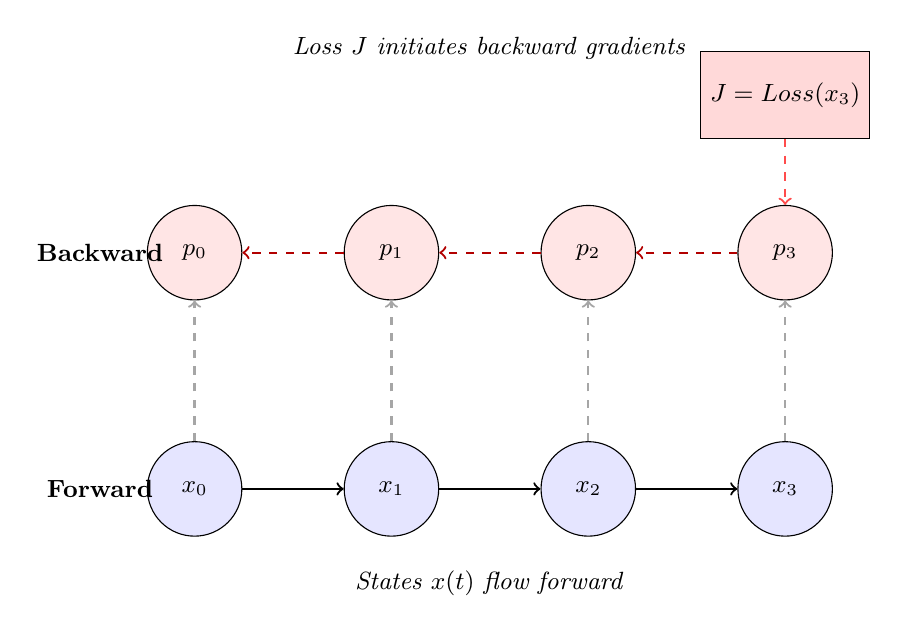
\begin{tikzpicture}[every node/.style={transform shape}, node distance=2cm and 1cm, font=\small]

  % Adjusted y-coordinates for vertical spacing
  \def\yForward{0}
  \def\yBackward{3}
  \def\yLoss{5}

  % Forward activations (state x)
  \node[circle, draw, fill=blue!10, minimum size=1.2cm] (x0) at (0, \yForward) {\(x_0\)};
  \node[circle, draw, fill=blue!10, minimum size=1.2cm] (x1) at (2.5, \yForward) {\(x_1\)};
  \node[circle, draw, fill=blue!10, minimum size=1.2cm] (x2) at (5, \yForward) {\(x_2\)};
  \node[circle, draw, fill=blue!10, minimum size=1.2cm] (x3) at (7.5, \yForward) {\(x_3\)};

  % Loss node J
  \node[rectangle, draw, fill=red!15, minimum width=1.6cm, minimum height=1.1cm] (loss) at (7.5, \yLoss) {\(J = \text{Loss}(x_3)\)};

  % Backpropagated gradients p(t)
  \node[circle, draw, fill=red!10, minimum size=1.2cm] (p3) at (7.5, \yBackward) {\(p_3\)};
  \node[circle, draw, fill=red!10, minimum size=1.2cm] (p2) at (5, \yBackward) {\(p_2\)};
  \node[circle, draw, fill=red!10, minimum size=1.2cm] (p1) at (2.5, \yBackward) {\(p_1\)};
  \node[circle, draw, fill=red!10, minimum size=1.2cm] (p0) at (0, \yBackward) {\(p_0\)};

  % Forward arrows (left to right)
  \draw[->, thick] (x0) -- (x1);
  \draw[->, thick] (x1) -- (x2);
  \draw[->, thick] (x2) -- (x3);

  % Backward arrows (right to left)
  \draw[->, thick, dashed, red!70!black] (p3) -- (p2);
  \draw[->, thick, dashed, red!70!black] (p2) -- (p1);
  \draw[->, thick, dashed, red!70!black] (p1) -- (p0);

  % Vertical dashed arrows from x to p
  \draw[->, thick, dashed, gray!70] (x3) -- (p3);
  \draw[->, thick, dashed, gray!70] (x2) -- (p2);
  \draw[->, thick, dashed, gray!70] (x1) -- (p1);
  \draw[->, thick, dashed, gray!70] (x0) -- (p0);

  % Loss injects gradient into p3
  \draw[->, thick, dashed, red!70] (loss) -- (p3);

  % Labels
  \node at (-1.2, \yForward) {\textbf{Forward}};
  \node at (-1.2, \yBackward) {\textbf{Backward}};
  \node at (3.75, \yForward - 1.2) {\small \textit{States \(x(t)\) flow forward}};
  \node at (3.75, \yLoss + 0.6) {\small \textit{Loss \(J\) initiates backward gradients}};
\end{tikzpicture}
\caption{Expanded vertical layout of training dynamics. States evolve forward through the network, while the loss initiates backward feedback via costates \(p(t)\) that guide learning.}
\end{figure}



\paragraph{Example.} Let’s say we’re training a neural network to recognize handwritten digits using the MNIST dataset. The output layer \(\mathbf{x}(3)\) contains 10 neurons—one for each digit class. For a given input image, the network produces the following output probabilities after softmax:

\[
\mathbf{x}(3) = 
\begin{bmatrix}
0.05 & 0.02 & 0.10 & 0.01 & \mathbf{0.60} & 0.04 & 0.05 & 0.03 & 0.06 & 0.04
\end{bmatrix}
\]

Here, the model predicts class 4 with the highest confidence (\(60\%\)). But suppose the true label is 2. We compute the cross-entropy loss:

\[
J = -\log(\mathbf{x}_3[2]) = -\log(0.10) \approx 2.30
\]

This high loss reflects a poor prediction—the model was confident, but confidently wrong. This scalar value \(J\) now drives the learning process:

\begin{enumerate}
	\item It initiates the backward pass.
	\item It generates gradients that ripple back through the network.
	\item It tells the optimizer how to adjust the weights to reduce future error.
\end{enumerate}

In this light, \(J\) isn’t just an error—it’s a signal with purpose. It encodes the task-specific notion of success and becomes the origin point of all correction in the learning loop.

Just as a compass doesn’t move the traveler but tells them where they should go, the loss function doesn’t directly change the network—it tells the optimizer how to reshape the landscape so future paths align with the desired goal.

\begin{figure}[H]
\centering
\begin{tikzpicture}[every node/.style={transform shape}, font=\small, node distance=2cm and 1cm]

  % Output layer label
  \node at (-2.3, 7.8) {\textbf{Output Layer:} \(\mathbf{x}(3)\)};

  % Output layer activations (with more vertical spacing)
  \node[circle, draw, fill=blue!10, minimum size=1cm] (x1) at (0, 7.2) {\(0.05\)};
  \node[circle, draw, fill=blue!10, minimum size=1cm] (x2) at (0, 5.7) {\(0.02\)};
  \node[circle, draw=red!70!black, very thick, fill=blue!10, minimum size=1cm] (x3) at (0, 4.2) {\(0.10\)};
  \node[circle, draw, fill=blue!10, minimum size=1cm] (x4) at (0, 2.7) {\(0.01\)};
  \node[circle, draw, fill=blue!10, minimum size=1cm] (x5) at (0, 1.2) {\(0.60\)};

  % Loss block
  \node at (6, 8.0) {\textbf{Loss Function}};
  \node[rectangle, draw, fill=red!15, minimum width=3.2cm, minimum height=1.2cm] (loss) at (6, 4.2) {\(J = -\log(0.10) \approx 2.30\)};
  \node[below=0.3cm of loss, align=center] {\footnotesize Cross-Entropy Loss \\[-0.2em] \footnotesize for true class = 2};

  % Arrow from selected activation to loss
  \draw[->, thick, red!70!black] (x3) -- node[above, sloped, font=\scriptsize] {\textcolor{red!60!black}{true label prob}} (loss);

  % Label next to selected class
 \node[font=\scriptsize, align=left, text width=4cm] at ([xshift=-3cm]x3) 
  {\textcolor{red!70!black}{True class (index 2) selected.\\Loss is \(-\log(x_3)\).}};


  % Clear caption below figure
\node[align=left, text width=10cm] at (2.2, -0.4) 
  {\footnotesize \textit{Cross-entropy loss penalizes low confidence in the correct class.\\The output \(x_3 = 0.10\) leads to a loss of \(-\log(0.10)\).}};



\end{tikzpicture}
\caption{The objective \(J\) compares the network output \(\mathbf{x}(3)\) to the true label using cross-entropy. A confident prediction yields low loss; a weak prediction (as here) yields higher loss.}
\end{figure}



\subsection{How the West Won the Feedback Loop (and Monetized It)}

Pontryagin's equations were designed to power rockets, regulate economies, and help central planners outmaneuver capitalist chaos. In the USSR, control theory was political: mathematics as command and control, not just description. 

\textbf{Cut to:} The present.

\begin{quote}
When Pontryagin wrote \( H(x, u, p, t) = p^\top f(x, u, t) + L(x, u, t) \), 
he thought it would help steer the future of humanity.  
Google read that and said, `'`Nice. Let’s use it to target ads during pregnancy.''
\end{quote}

Control theory wasn’t supposed to tell you which ad to click; it was supposed to tell the future where to go.

\begin{itemize}
  \item Deep learning? That’s just optimal control in disguise. 
  \item The forward pass? A corporate strategy. 
  \item Backpropagation? A shadow price. 
  \item Loss minimization? Economic planning—except; instead of a five-year plan, it’s a five-millisecond attention grab.
\end{itemize}

Meanwhile, hedge funds now run control-theoretic models on GPUs faster than Soviet computers could boot up. Every gradient is a potential arbitrage. Every costate is a profit signal. The whole economic apparatus is backpropagated.

The West did not ignore Pontryagin’s dream. No, they optimized it... for money.

\textbf{Narrator (Ron Howard's voice):}  
\emph{He had, in fact, built the perfect capitalist machine.}

In the end, the mathematics Pontryagin meant to overthrow markets ended up running them. And, the dialectic didn’t just turn; it got monetized.

\begin{quote}
\emph{The observer is no longer just active... he is very, very well-funded.}
\end{quote}





\begin{figure}[H]
  \centering
  
  % === First row ===
  \begin{subfigure}[t]{0.45\textwidth}
  \centering
  \begin{tikzpicture}
    \comicpanel{0}{0}
      {Pontryagin}
      {}
      {\footnotesize This system will guide workers to prosperity.}
      {(0,-0.6)}
  \end{tikzpicture}
  \caption*{Control theory for socialism.}
  \end{subfigure}
  \hfill
  \begin{subfigure}[t]{0.45\textwidth}
  \centering
  \begin{tikzpicture}
    \comicpanel{0}{0}
      {Google}
      {}
      {\footnotesize We use the same math to predict baby food purchases before the second trimester.}
      {(0,-0.6)}
  \end{tikzpicture}
  \caption*{Control theory for capitalism.}
  \end{subfigure}
  
  \vspace{1em}
  
  % === Second row ===
  \begin{subfigure}[t]{0.45\textwidth}
  \centering
  \begin{tikzpicture}
    \comicpanel{0}{0}
      {Pontryagin}
      {}
      {\footnotesize The Hamiltonian should optimize national progress!}
      {(0,-0.6)}
  \end{tikzpicture}
  \caption*{His equations haunt silicon.}
  \end{subfigure}
  \hfill
  \begin{subfigure}[t]{0.45\textwidth}
  \centering
  \begin{tikzpicture}
    \comicpanel{0}{0}
      {Wall Street}
      {}
      {\footnotesize Every costate is a trading signal. Every gradient is a payday.}
      {(0,-0.6)}
  \end{tikzpicture}
  \caption*{The maximum principle becomes a revenue model.}
  \end{subfigure}
  
  \caption{Pontryagin dreamed of optimal control for human futures. The West backpropagated that dream... into quarterly profits.}
  \end{figure}
  